\documentclass[a4paper,12pt,openany,oneside]{book}
\usepackage[a4paper,top=2cm,bottom=2cm,left=2cm,right=3cm]{geometry}
\usepackage{courier}
\renewcommand*\familydefault{\ttdefault} %% Only if the base font of the document is to be typewriter style
\usepackage[T1]{fontenc}
\usepackage[T1]{fontenc}
\usepackage[utf8]{inputenc}
\usepackage[italian]{babel}
\usepackage[colorlinks,linkcolor=black]{hyperref}%linked package
\usepackage[font={small}]{caption}
\usepackage[rightcaption]{sidecap}
\usepackage{graphicx}
\graphicspath{ {images/} }
\usepackage{listings}
\usepackage{xcolor}
\usepackage{minted}

\setcounter{tocdepth}{3}
\setcounter{secnumdepth}{3}

%\usepackage{imakeidx}
%\makeindex

\definecolor{codegreen}{rgb}{0,0.6,0}
\definecolor{codegray}{rgb}{0.5,0.5,0.5}
\definecolor{codepurple}{rgb}{0.58,0,0.82}
\definecolor{backcolour}{rgb}{0.95,0.95,0.92}

\lstdefinestyle{mystyle}{
    backgroundcolor=\color{backcolour},   
    commentstyle=\color{magenta},
    keywordstyle=\color{codegreen},
    numberstyle=\tiny\color{codegray},
    stringstyle=\color{codepurple},
    basicstyle=\ttfamily\footnotesize,
    breakatwhitespace=false,         
    breaklines=true,                 
    captionpos=b,                    
    keepspaces=true,                 
    numbers=left,                    
    numbersep=5pt,                  
    showspaces=false,                
    showstringspaces=false,
    showtabs=false,                  
    tabsize=2
}

\lstset{style=mystyle}

%font 
\usepackage{cochineal}

\title{Documentazione App Vaccinazioni }
\author{Andrei Lazar & Lorenzo Bonanni }
\date{Luglio 2021}

\setcounter{secnumdepth}{-2} 
\begin{document}
\maketitle
\pagestyle{plain}
\tableofcontents
\newenvironment{citazione}[1]
  {\newcommand{\lafonte}{#1}%
   \begin{quotation}}
  {\par\nobreak\raggedleft\relax[\lafonte]
   \end{quotation}}


% \chapter*{Note generali}
% Il progetto é stato commissionato a un magrebino indiano sottopagato rigiorsamente é con skill minor delle nostre il progetto nel complesso é uscito una copia spudurata sel portale USSL 9 rigorsamente voluto 
\chapter{Requisiti ed interazioni utente-sistema}
\section{Specifiche casi d’uso}
\begin{figure}[h]
\centering
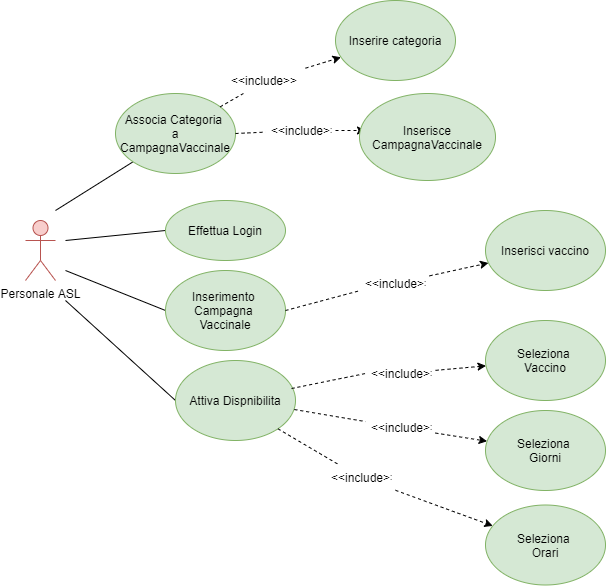
\includegraphics[width=0.4\columnwidth]{asl.png} 
\caption{caso d'uso relativo al personale ASL} 
\end{figure}
\subsection{Casi d'uso relativo al Personale ASL}
\subsubsection*{Effetuare login}
Il personale Asl si indentifica mediante una parola/codice segreto tramite l'intefaccia generica di login\\
\fbox{\begin{minipage}{lung}
\textbf{Attori:} ASL\\
\textbf{Precodizioni:} Nessuna\\
\textbf{Passi:}
\begin{itemize}
  \item Il personale accede al sistema 
  \item Il personale è introdotto al interfaccia di base
\end{itemize}
\textbf{Postcondizioni:} Il personale puo accedere alle varie sezioni elencate
\end{minipage}}

\subsubsection*{Inserimento campagne vaccinali}
Il sistema di prenotazione è gestito dal personale dell’ASL, che può inserire la campagna vaccinale di volta in volta considerata (influenza, Covid-19, SarS, e così via).\\
\fbox{\begin{minipage}{37em}
\textbf{Attori:} ASL\\
\textbf{Precodizioni:} Il personale deve aver effettuato l'accesso\\
\textbf{Passi:}
\begin{itemize}
  \item Il personale seleziona l'optione "Aggiungi Campagna vaccinale" 
  \item Il personale aggiunge i vaccini relativi alla campagna vaccinale
  \item Il personale inserisce il nome della malattia 
\end{itemize}
\textbf{Postcondizioni:} Il personale é introdotto al intefaccia di base
\end{minipage}}

\subsubsection*{Inserimento scorte vaccini}
Il personale ASL puo andare a modificare le scorte relative a uno specifico vaccino.\\
\fbox{\begin{minipage}{37em}
\textbf{Attori:} ASL\\
\textbf{Precodizioni:} Il personale deve aver effettuato l'accesso\\
\textbf{Passi:}
\begin{itemize}
  \item Il personale clicca il pulsante "Modifica Scorte Vaccino" 
  \item Il personale seleziona il vaccino a cui aggiungere scorte
  \item Il personale inserisce la quantità da aggiungere
\end{itemize}
\textbf{Postcondizioni:} Il personale é introdotto al intefaccia di base
\end{minipage}}

\subsubsection*{Inserimento Disponibilitá}
Il personale ASL può aggiungere date nelle quali è possibile vaccinarsi\\
\fbox{\begin{minipage}{37em}
\textbf{Attori:} ASL\\
\textbf{Precodizioni:} Il personale deve aver effettuato l'accesso\\
\textbf{Passi:}
\begin{itemize}
  \item Il personale clicca il pulsante "Aggiungi Disponibilità"
  \item Il personale seleziona il vaccino 
  \item Il personale inserisce i dati relativi alla disponibilità
\end{itemize}
\textbf{Postcondizioni:} Il personale é introdotto al intefaccia di base
\end{minipage}}
\subsubsection*{Inserimento Categoria vaccino}
Il personale ASL associa ad ogni campagna vaccinale le categorie di cittadini che hanno diritto alle vaccinazioni con uno specifico vaccino.\\
\fbox{\begin{minipage}{37em}
\textbf{Attori:} ASL\\
\textbf{Precodizioni:} Il personale deve aver effettuato l'accesso\\
\textbf{Passi:}
\begin{itemize}
  \item Il personale clicca il pulsante "Associa Vaccino a Categoria"
  \item Il personale seleziona il vaccino
  \item Il personale seleziona la Categoria
\end{itemize}
\textbf{Postcondizioni:} Il personale é introdotto al intefaccia di base
\end{minipage}}
\newpage
%Utente
\subsection{Casi d'uso relativo al Utente}
%IMMAGINE
\begin{figure}[h] 
\centering
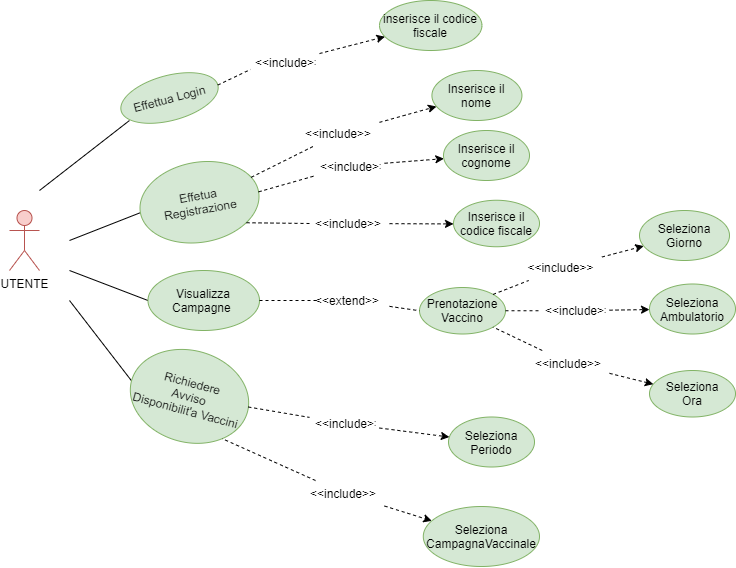
\includegraphics[width=0.6\columnwidth]{utente.png} 
\caption{caso d'uso relativo al Utente} 
\end{figure}
\subsubsection*{Schermata iniziale}
I cittadini che aderiscono ad una certa campagna vaccinale possono accedere al sistema di prenotazione dopo essersi registrati. In fase di registrazione, essi devono indicare nome, cognome, codice fiscale, e saranno informati della specifica categoria di appartenenza (“over 80”, “età 70-79”, “paziente oncologico”, “paziente iperteso”, “paziente a rischio”, e così via), di cui il sistema è a conoscenza\\\\
\fbox{\begin{minipage}{37em}
\textbf{Attori:} Utente\\
\textbf{Precodizioni:} Utente non registrato\\
\textbf{Passi:}
\begin{itemize}
  \item Inserire codice fiscale e confermare
\end{itemize}
\textbf{Postcondizioni:} Utente introdotto al intefaccia di registrazione
\end{minipage}}

\subsubsection*{Schermata Registrazione}
\fbox{\begin{minipage}{37em}
\textbf{Attori:} Utente\\
\textbf{Precodizioni:} L'utente deve essersi identificato tramite codice fiscale\\
\textbf{Passi:}
\begin{itemize}
  \item L'utente inserisce il nome
  \item L'utente inserisce il cognome
  \item L'utente inserisce il codice fiscale
\end{itemize}
\textbf{Postcondizioni:} L'utente riceve il feedback di registrazione e gli viene comunicata la categoria di appartenenza.
\end{minipage}}
\subsubsection*{Visualizza Campagne}
Una volta registrati, i cittadini accedono al  e trovano le campagne vaccinali a cui possono aderire.
\fbox{\begin{minipage}{37em}
\textbf{Attori:} Utente\\
\textbf{Precodizioni:} Utente ha effettuato il login\\
\textbf{Passi:}
\begin{itemize}
  \item Utente seleziona la campagna di interesse
\end{itemize}
\textbf{Postcondizioni:} L'utente é introdotto al interfaccia di disponibilita luogo
\end{minipage}}
\subsubsection*{Visualizza Disponibilita Luogo}
Per ogni campagna il cittadino può vedere gli orari e le sedi disponibili giorno per giorno e
selezionare il momento desiderato presso l’ambulatorio che desidera.\\
\fbox{\begin{minipage}{37em}
\textbf{Attori:} Utente\\
\textbf{Precodizioni:} Utente ha scelto una campagna \\
\textbf{Passi:}
\begin{itemize}
  \item L'utente seleziona luogo 
  \item L'utente conferma
\end{itemize}
\textbf{Postcondizioni:} l'utente viene indirizzato alla schermata di scelta del giorno 
\end{minipage}}
\subsubsection*{Visualizza Disponibilita Giorno}
Per ogni campagna il cittadino può vedere gli orari e le sedi disponibili giorno per giorno e
selezionare il momento desiderato presso l’ambulatorio che desidera.\\
\fbox{\begin{minipage}{37em}
\textbf{Attori:} Utente\\
\textbf{Precodizioni:} Utente ha scelto un luogo  \\
\textbf{Passi:}
\begin{itemize}
  \item L'utente seleziona un giorno disponible   
  \item L'utente seleziona una ora disponibile 
  \item L'utente conferma prenotazione
\end{itemize}
\textbf{Postcondizioni:} l'utente riceve conferma grafica della prenotazione 
\end{minipage}}

\newpage
%SISTEMA 
\subsection{Casi d'uso relativo al Sistema}

%IMMAGINE 
\begin{figure}[h] 
\centering
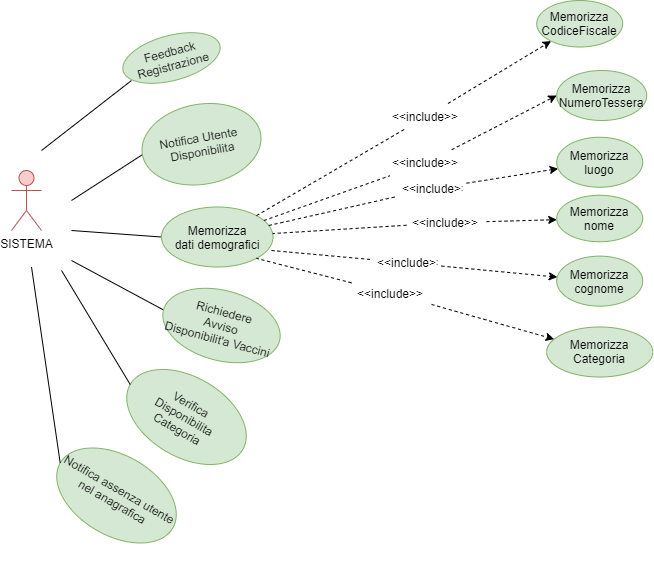
\includegraphics[width=0.6\columnwidth]{sistema.png} 
\caption{caso d'uso relativo al Sistema} 
\end{figure}

\subsection*{Sistema}
l sistema memorizza i dati demografici essenziali per ogni cittadino: codice fiscale, numero di
tessera sanitaria, cognome, nome, luogo e data di nascita, specifiche categorie appartenenza
(paziente oncologico, paziente iperteso, paziente a rischio, e così via)\\
\fbox{\begin{minipage}{37em}
\textbf{Attori:} Sistema\\
\textbf{Precodizioni:}  Nessuna\\
\textbf{Passi:}
\begin{itemize}
  \item Il sistema memorizza i dati demografici
\end{itemize}
\textbf{Postcondizioni:} I dati demografici sono stati salvati
\end{minipage}}
\subsubsection*{Notifica Disponibilità}
Il sistema avvisa il cittadino, che ne abbia fatto richiesta attraverso il sistema, rispetto al momento in cui un certo periodo di tempo sarà disponibile per le prenotazioni di una data campagna vaccinale.\\
\fbox{\begin{minipage}{37em}
\textbf{Attori:} Utente, Sistema, Personale\\
\textbf{Precodizioni:} 
\begin{itemize}
  \item L'utente ha fatto richiesta di essere notificato
  \item Il personale ASL ha insertito una disponibilità compatibile con la richiesta dell'utente
  \item L'utente ha effettuato il login
\end{itemize}
\textbf{Passi:}
\begin{itemize}
  \item Il sistema notifica l'utente 
\end{itemize}
\textbf{Postcondizioni:} L'utente è introdotto al interfaccia di base
\end{minipage}}
%TO DO DA FARE!!
\section{Sequence diagram di dettaglio per i principali Use Case}
\subsection*{Note Generali}
Il Sequence Diagram permette di modellare le interazioni tra attori e oggetti e di gestire i requisiti che cambiano durante il processo e sviluppo del sistema.
\subsection{Utente}
Nel caso dell'utente abbiamo:
\begin{itemize}
  \item Prenotazione Vaccino
  \item Registrazione
  \item Login
\end{itemize}
%IMMAGINE 
\begin{figure}[h] 
\centering
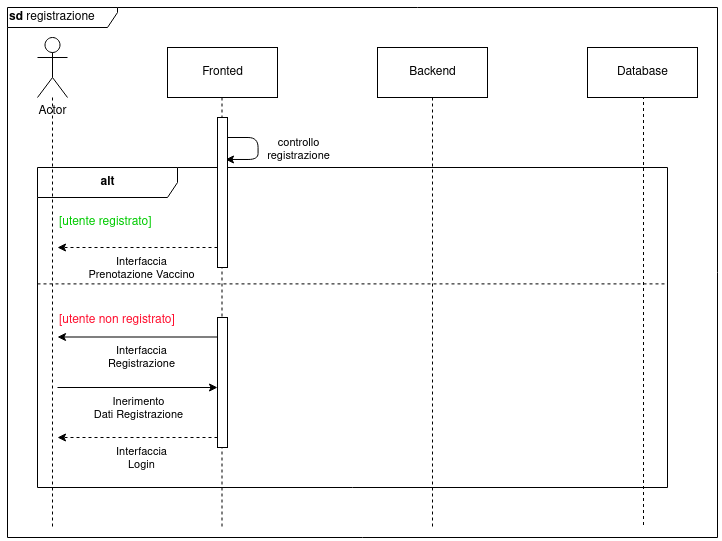
\includegraphics[width=0.8\columnwidth]{Registration.png} 
\caption{Sequence Diagram Utente Registrazione} 
\end{figure}
\newpage
%IMMAGINE 
\begin{figure}[h] 
\centering
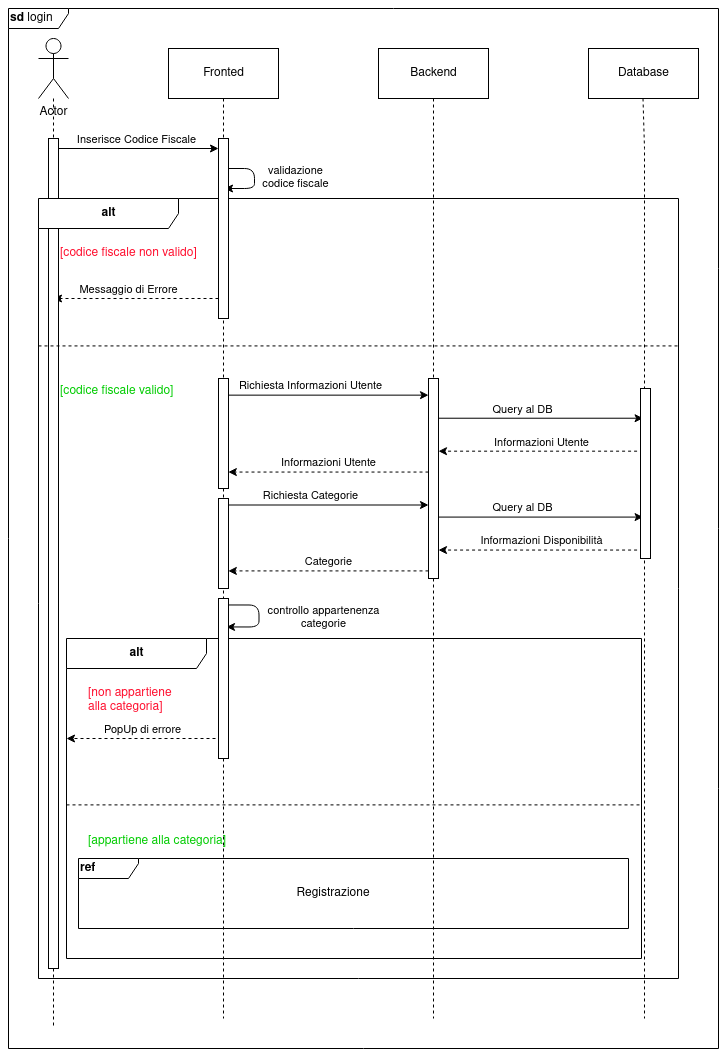
\includegraphics[width=0.8\columnwidth]{Authentication-Page-1.png} 
\caption{Sequence Diagram Utente Login}
\end{figure}
\newpage
%IMMAGINE 
\begin{figure}[h] 
\centering
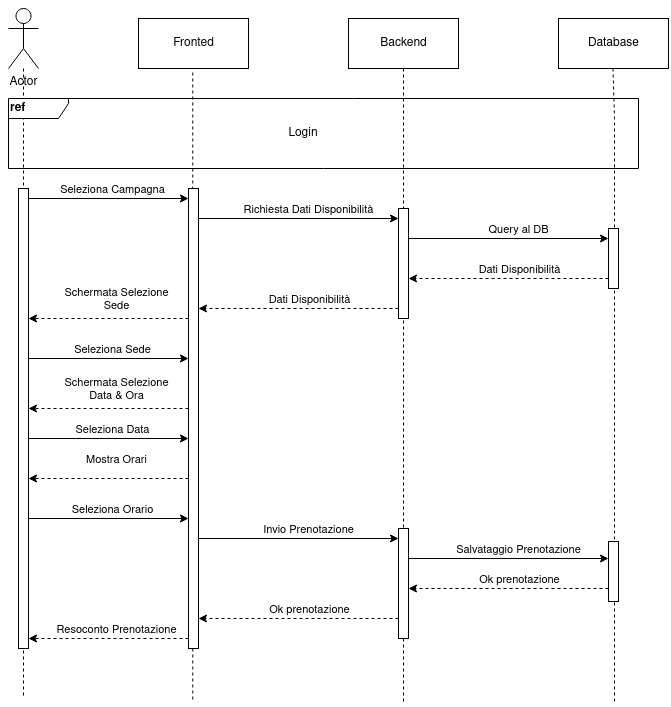
\includegraphics[width=0.8\columnwidth]{Stystem.png} 
\caption{Sequence Diagram Utente Prenotazione Vaccino} 
\end{figure}
\newpage

\subsection{Personale ASL}
Nel caso del personale ASL abbiamo un Sequence Diagram che rappresenta tutte le possibili operazioni che il personale può effettuare.
%IMMAGINE 
\begin{figure}[h] 
\centering
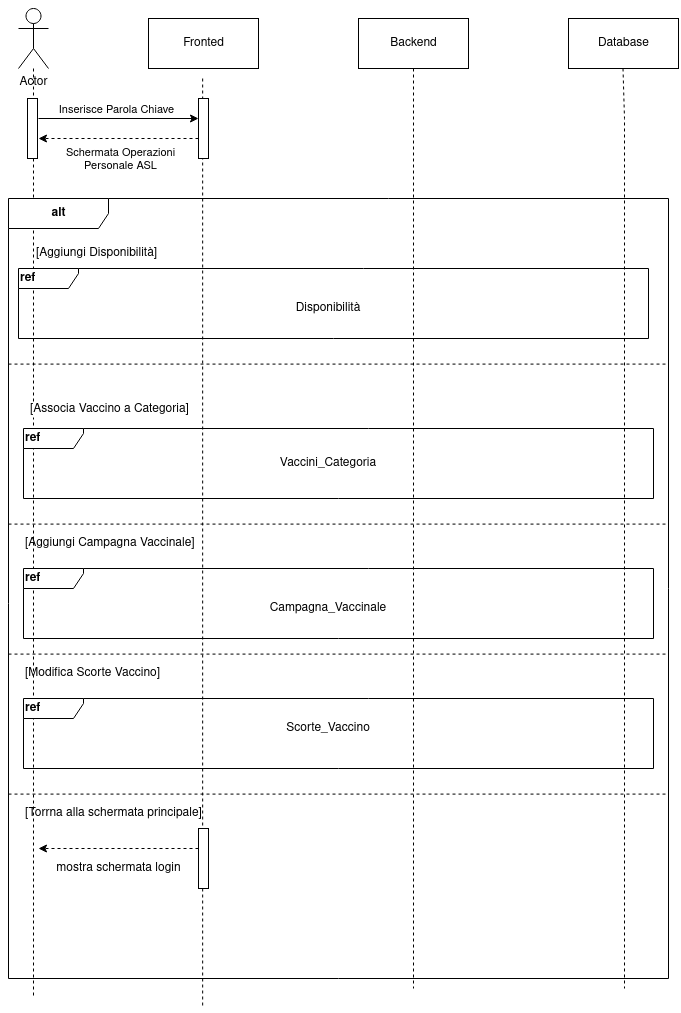
\includegraphics[width=0.8\columnwidth]{ASL-Personale-ASL.png} 
\caption{Personale-ASL} 
\end{figure}
%IMMAGINE 
\begin{figure}[h] 
\centering
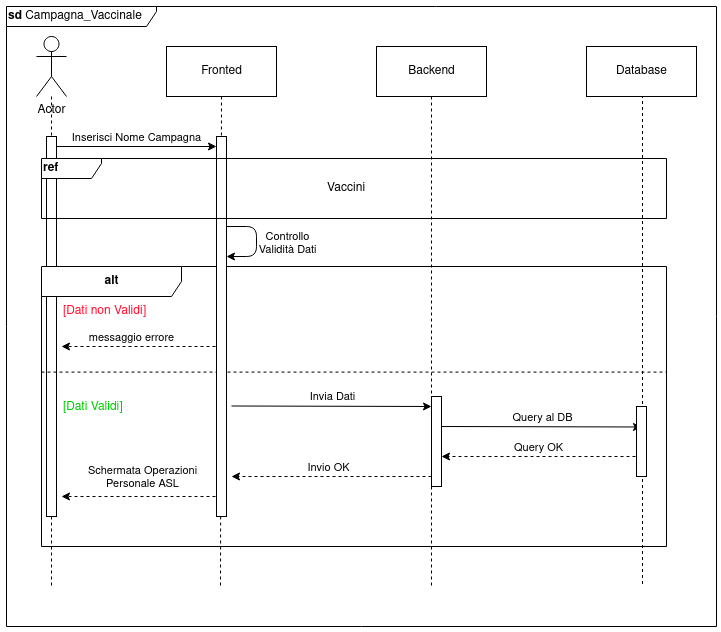
\includegraphics[width=0.8\columnwidth]{ASL-CAMPAGNA.png} 
\caption{ASL-CAMPAGNA} 
\end{figure}
%IMMAGINE 
\begin{figure}[h] 
\centering
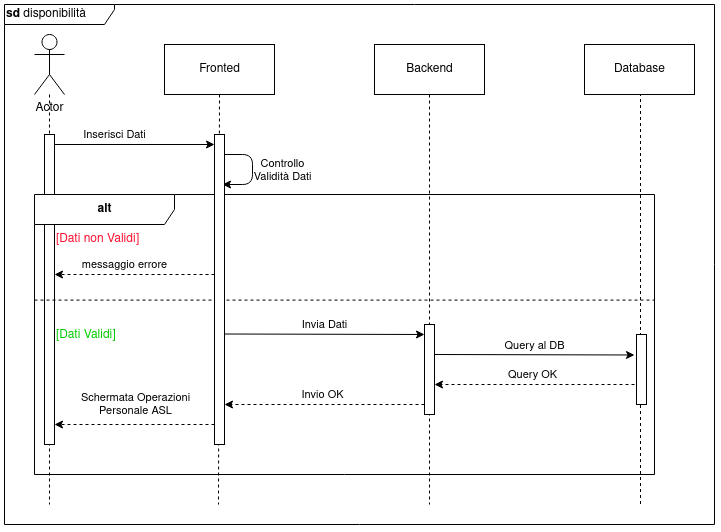
\includegraphics[width=0.8\columnwidth]{ASL-DISPONIBILITA.png} 
\caption{ASL-DISPONIBILITA} 
\end{figure}
%IMMAGINE 
\begin{figure}[h] 
\centering
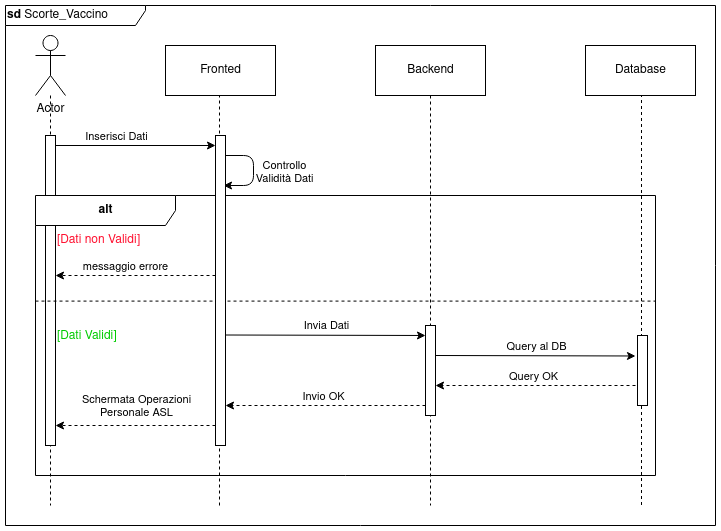
\includegraphics[width=0.8\columnwidth]{ASL-SCORTE.png} 
\caption{ASL-SCORTE} 
\end{figure}
%IMMAGINE 
\begin{figure}[h] 
\centering
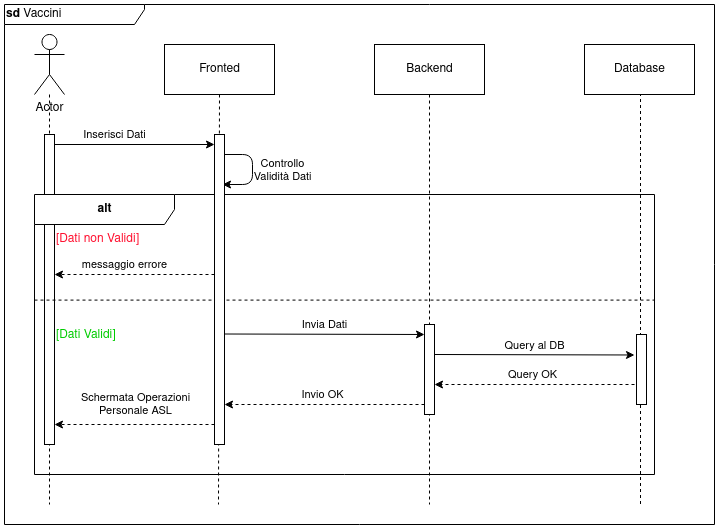
\includegraphics[width=0.8\columnwidth]{ASL-VACCINI.png} 
\caption{ASL-VACCINI} 
\end{figure}
%IMMAGINE 
\begin{figure}[h] 
\centering
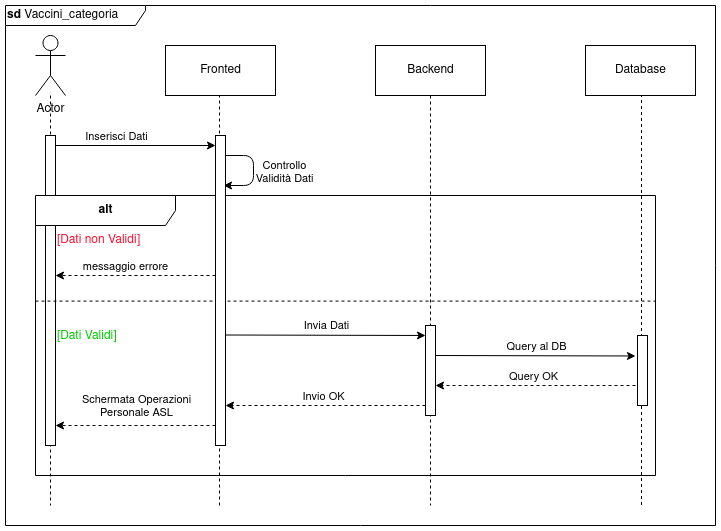
\includegraphics[width=0.8\columnwidth]{ASL-VACCINI CATEGORIA.png} 
\caption{ASL-VACCINI CATEGORIA} 
\end{figure}
\clearpage
\newpage
\section{Activity Diagram relativo alle modalità di interazione/operatività del
software}
\subsection*{Note Generali}
L’Activity Diagram modella un comportamento come un insieme di azioni organizzate secondo un
flusso.
\subsection{Utente}
Nel caso del \textbf{utente} si ha il seguente flusso di attivitá: L'utente inserisce il proprio codice fiscale, in  caso di registrazione già avvenuta visualizza la schermata con le campagne vaccinali altrimenti visualizza una scherma dove si registrerá.\\Nella Schermata delle campagne saranno visualizzate solo le campagne disponibili per la categoria in caso di assenza non verra mostrata la schermata ma un popup di errore.\\Selezionando la campagna l'utente verra indirizzato nella selezione delle sedi disponibili, una volta selezionata una sede verrà visualizzata una schermata con le date e i relativi pulsanti per impostare notifica, selezionare giorno, confermare prenotazione e tornare al login.
%IMMAGINE 
\begin{figure}[h] 
\centering
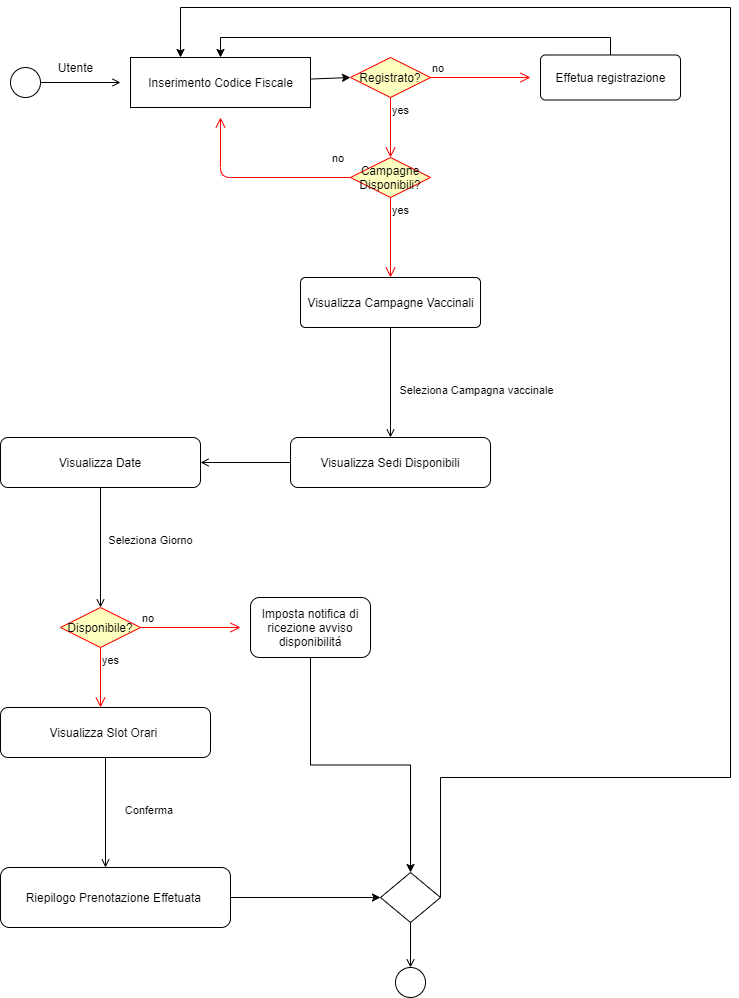
\includegraphics[width=0.6\columnwidth]{Activity Diagram Utente.png} 
\caption{Activity Diagram Utente} 
\end{figure}
\newpage
\subsection{ASL}
Nel caso del personale \textbf{asl} si ha il seguente flusso di attivitá: Il personale inserisce nella generica schermata di accesso la parola chiave per ottenere i privileggi una volta al interno della scherma sará possbile selezionare varie optioni : Aggiungi Disponibilitá, Associa Vaccino a Categoria, Aggiungi Campagna Vaccinale, Modifica Scorte Vaccino.\\
%IMMAGINE 
\begin{figure}[h] 
\centering
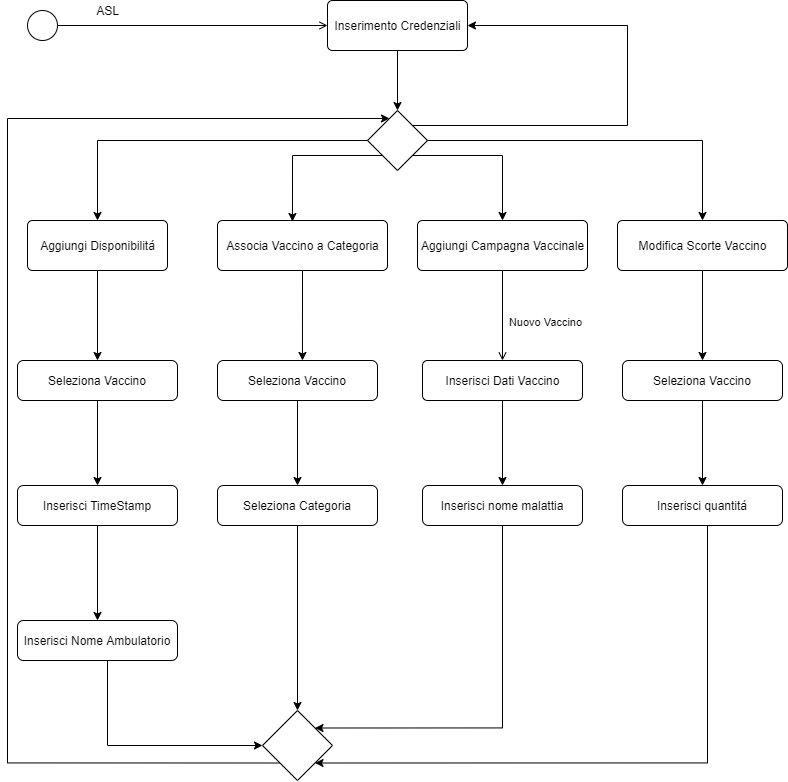
\includegraphics[width=0.5\columnwidth]{Activity Diagram ASL.png} 
\caption{Activity Diagram Asl} 
\end{figure}
\subsection{Sistema}
Nel caso del \textbf{Sistema} esso si occupa di tutta la parte logica e di controllo del elaborazione dei dati e il loro invio.
%IMMAGINE 
\begin{figure}[h] 
\centering
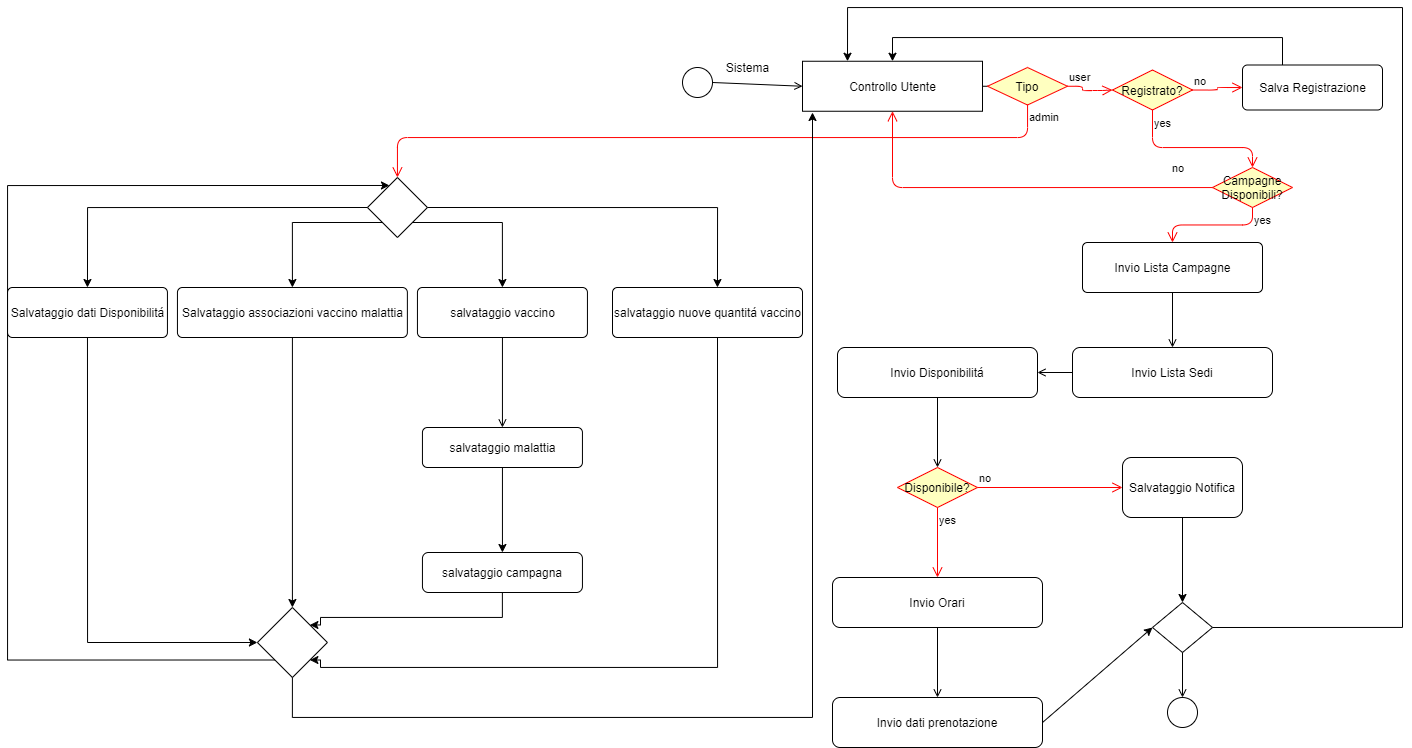
\includegraphics[width=0.8\columnwidth]{Activity Diagram Sistema.png} 
\caption{Activity Diagram sistema} 
\end{figure}
\newpage
\section{Class Diagram e Sequence diagram del software progettato}
\subsection*{Note Generali}
Il Class Diagram mostra le classi di oggetti nel sistema e le associazioni tra queste classi.
\subsection{Elenco campi entitá Model}
L’elenco dei campi rappresenta le classi con i loro rispettivi nomi, i predicati nominali, cioé i loro attributi. Gli attributi inseriti sono quelli richiesti dal progetto insieme ad altri attributi.
%IMMAGINE 
\begin{figure}[h] 
\centering
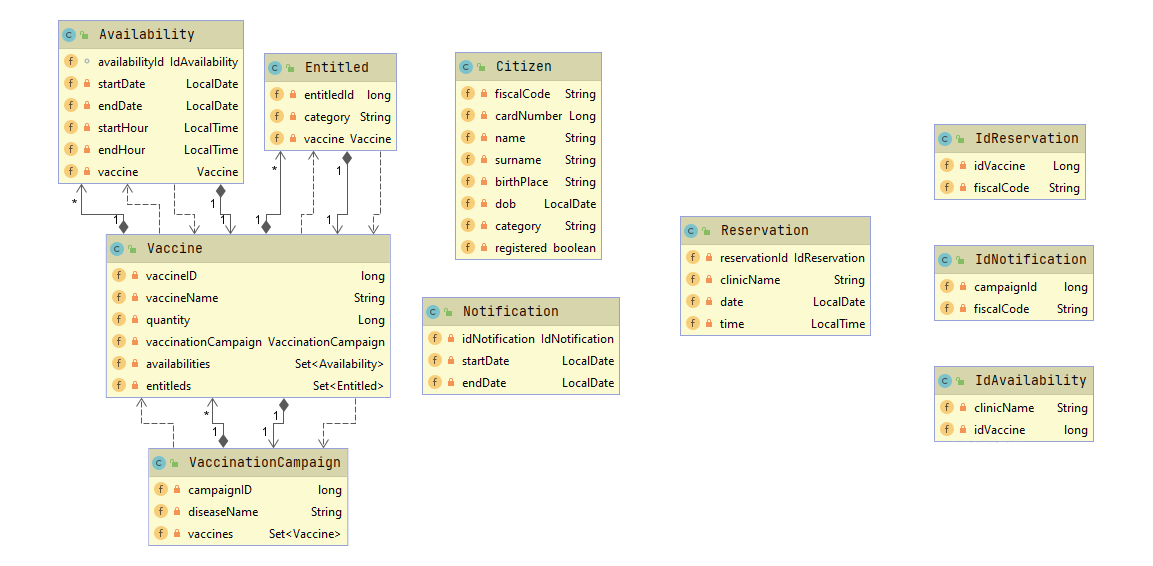
\includegraphics[width=0.9\columnwidth]{Package model.png} 
\caption{Model} 
\end{figure}
\subsection{Elenco metodi per ogni entità}
Per avere una maggiore leggibilitá del codice abbiamo adottato una classificazione delle entitá tramite package. Possiamo qui di seguito osservare una visione dei package del back-end
%IMMAGINE 
\begin{figure}[h] 
\centering
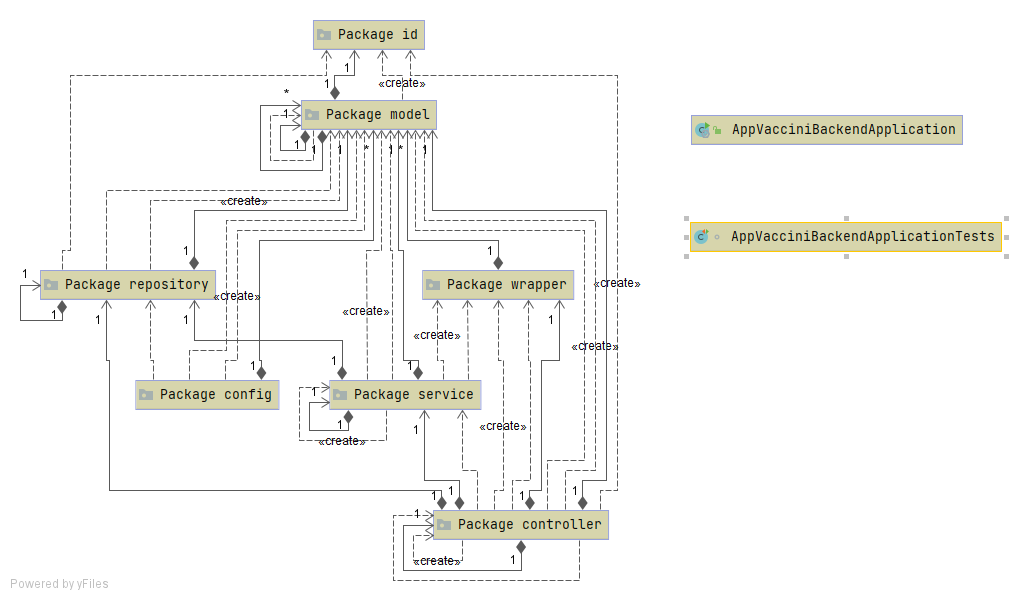
\includegraphics[width=0.8\columnwidth]{Package appvaccinibackend.png} 
\caption{Package appvaccinibackend} 
\end{figure}

%IMMAGINE 
\begin{figure}[h] 
\centering
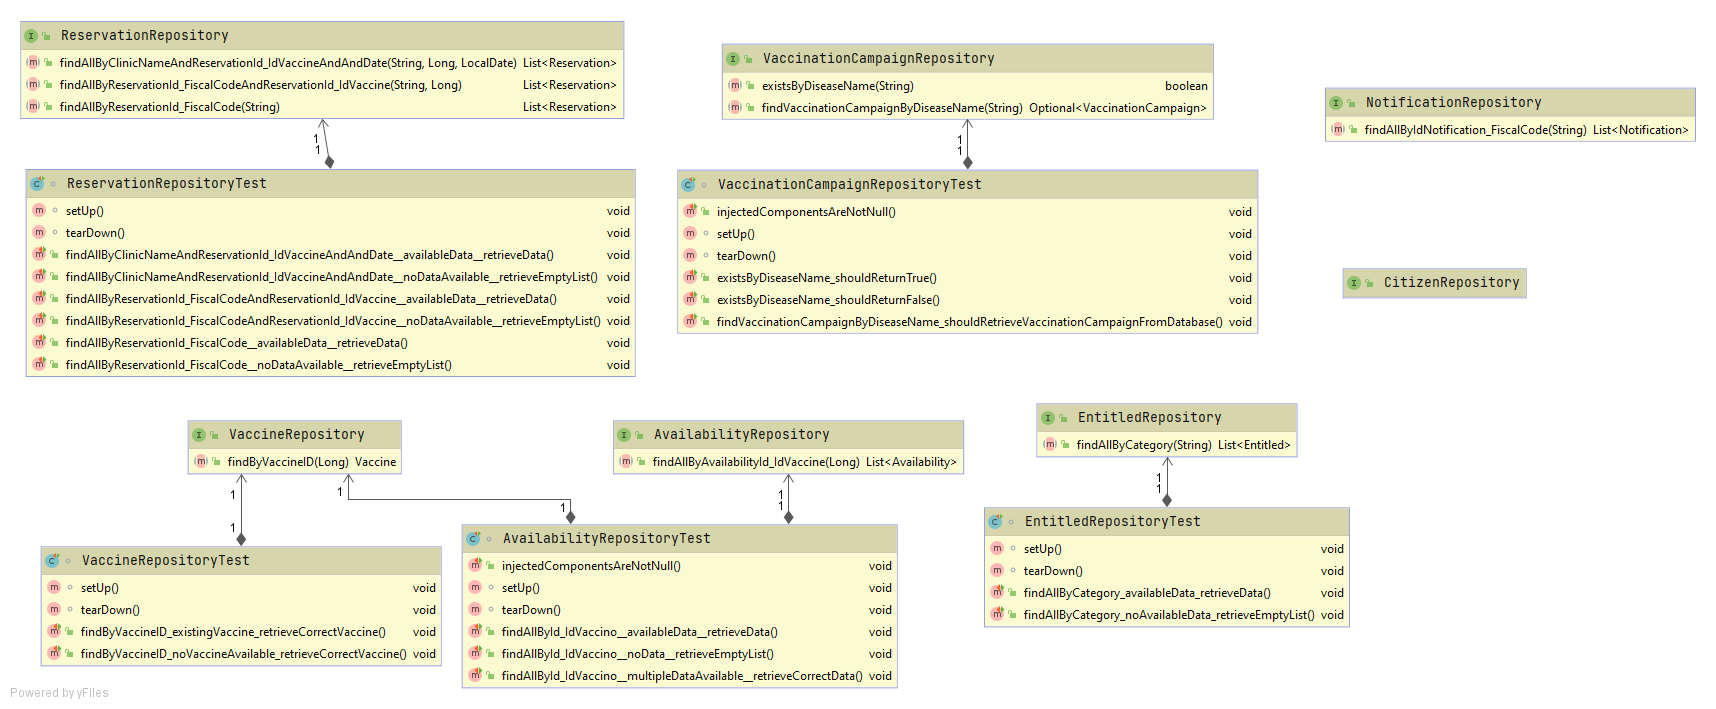
\includegraphics[width=0.8\columnwidth]{Package repository.png} 
\caption{Class Diagram Package repository} 
\end{figure}
%IMMAGINE 
\begin{figure}[h] 
\centering
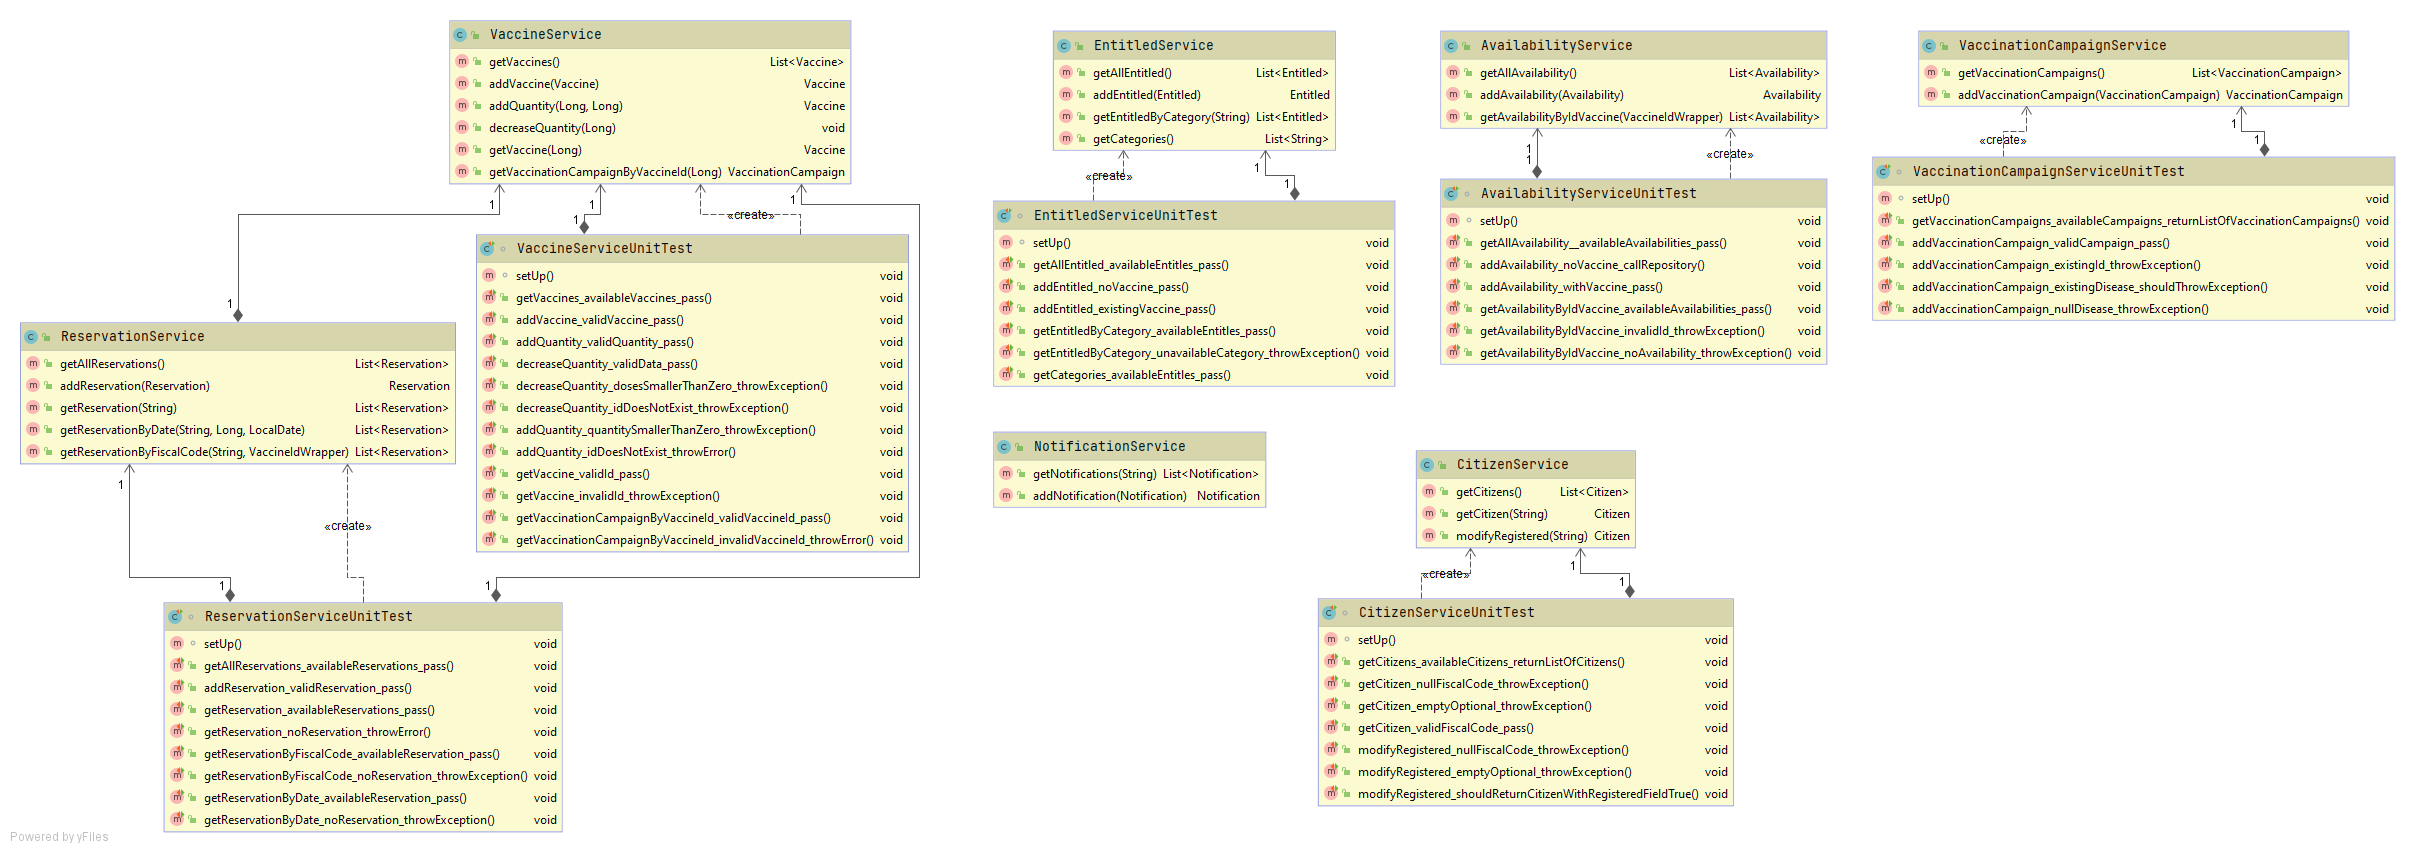
\includegraphics[width=1.2\columnwidth]{Package service.png} 
\caption{Class Diagram  Package service} 
\end{figure}
%IMMAGINE 
\begin{figure}[h] 
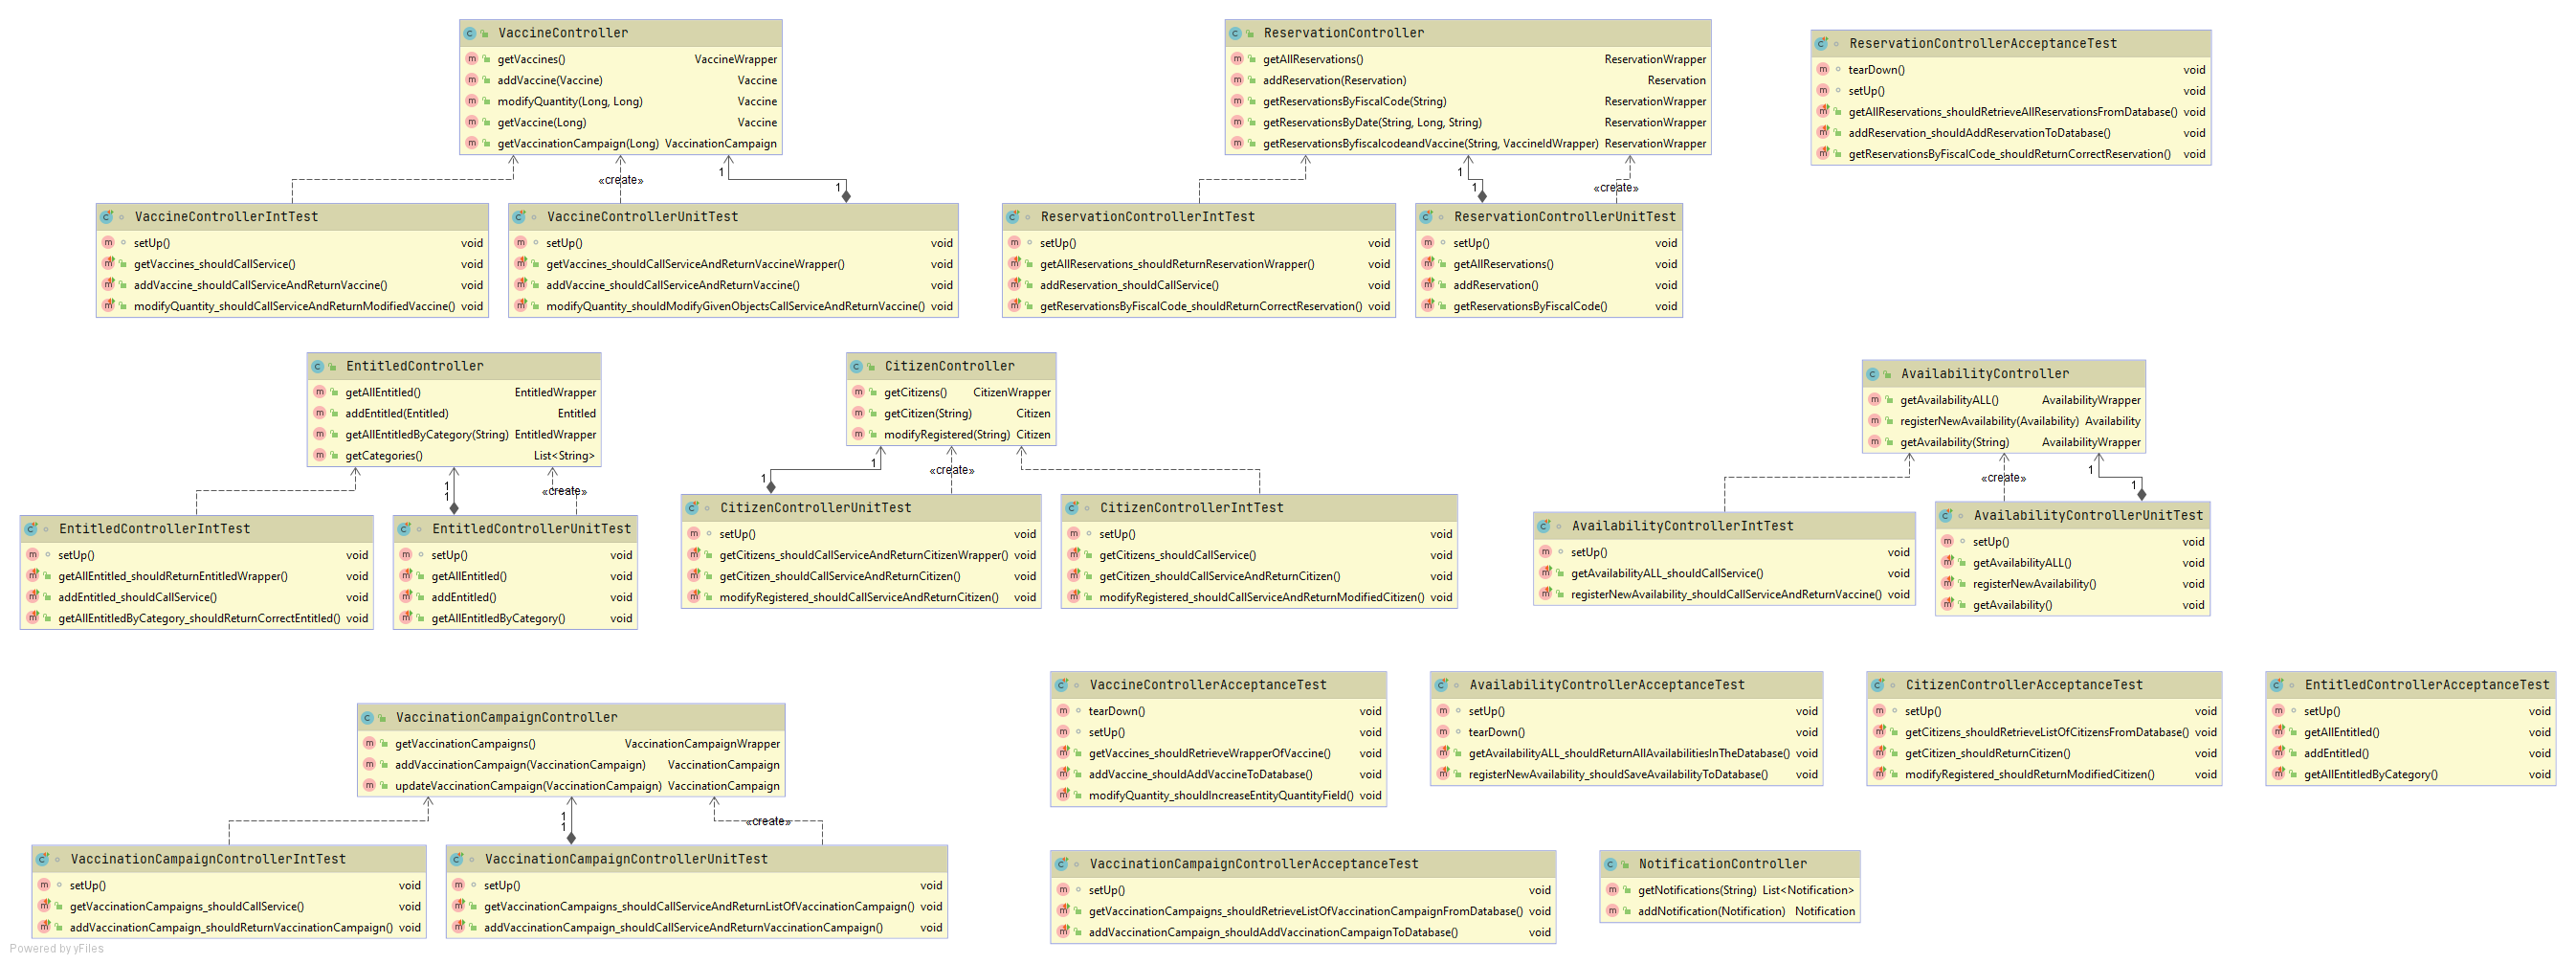
\includegraphics[width=1.2\columnwidth]{Package controller.png} 
\caption{Class Diagram Package controller} 
\end{figure}

%IMMAGINE 
\begin{figure}[h] 
\centering
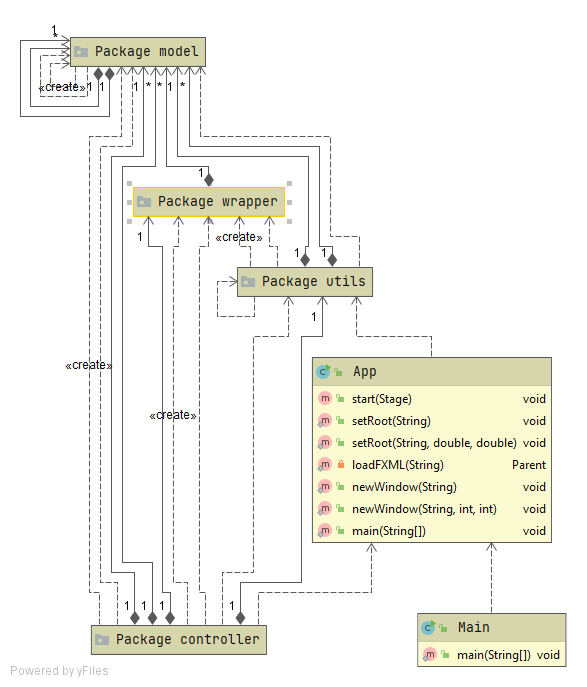
\includegraphics[width=0.6\columnwidth]{Package kodikasgroup Frontend.png} 
\caption{Package appvaccinifrontend} 
\end{figure}

%IMMAGINE 
\begin{figure}[h] 
\centering
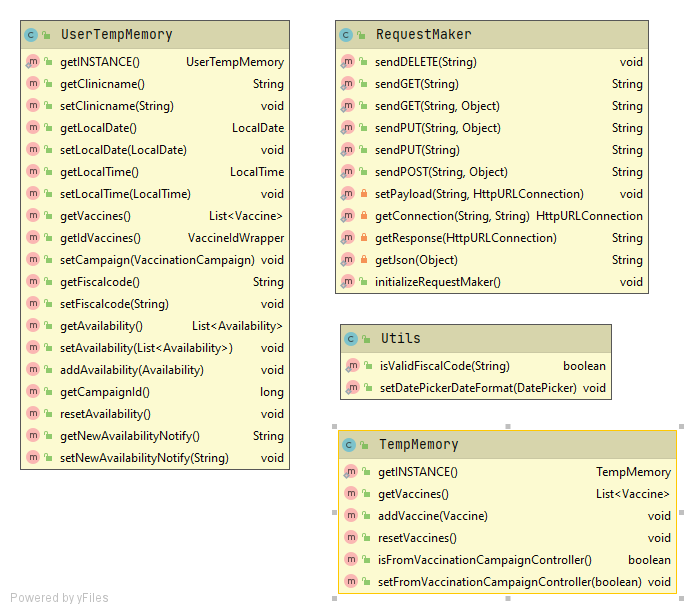
\includegraphics[width=0.8\columnwidth]{Package utils frontend.png} 
\caption{Package Utils Frontend} 
\end{figure}

%IMMAGINE 
\begin{figure}[h] 
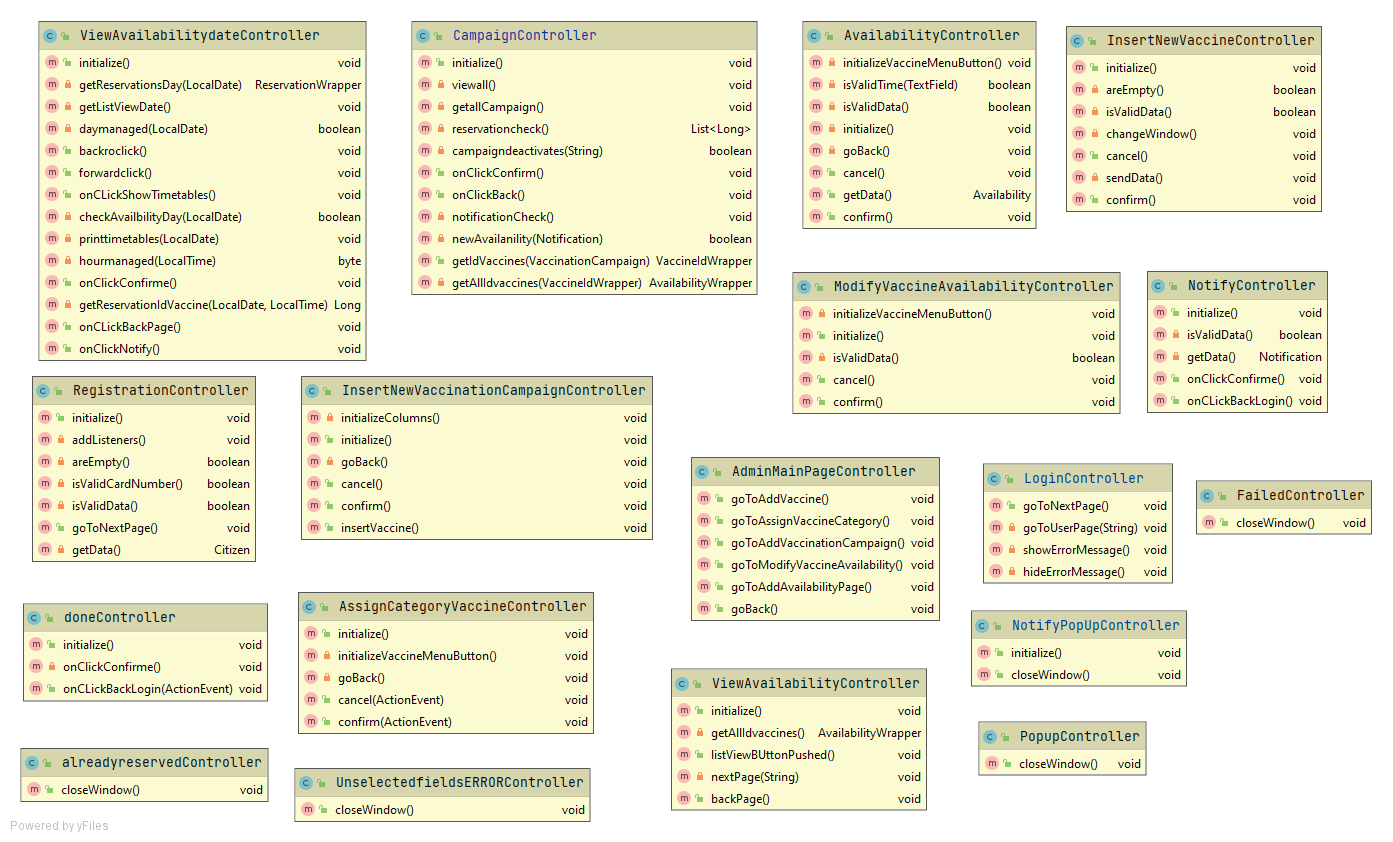
\includegraphics[width=1.1\columnwidth]{Package controller frontend.png} 
\caption{Package controller frontend} 
\end{figure}

\newpage
%CAP 2
\chapter{Sviluppo: {\\\normalfont Progetto dell'architettura ed implementazione del sistema}}
\section{Note sul processo di sviluppo }
Il processo di sviluppo é stato essenzialmente di tipo Plan-driven e incrementale  le attivitá sono state inzialmente programmate con una prima implementazione succesivamente perfezionata. Prima di inziare il processo di sviluppo c'è stata una fase iniziale di analisi dei requisiti , generando i relativi use-case e i diagrammi di attivitá.\\ Durante la pianificazione del processo di sviluppo è stata sfruttata una delle pecculiaritá di GitKraken, le  boards kanban dividendo appositamente in Backend, Frontend, To DO, Doing, Testing, Done a loro volta i contenenti dei processi stilati mediante analisi dei requisiti. \\Inoltre è stata usata anche un piattaforma per il versioning (GitHub). Dopo ogni sostanziale implementazione/versione sono stati eseguiti gli appositi test. Non sempre le fasi di sviluppo sono state lineari, infatti sono state intervallate da numerose attivitá di refectoring.

\section{Progettazione e pattern architetturali usati}
Il nostro progetto è stato sviluppato utilizzando un'architettura Client Server.
\subsection*{Client–server Architectural pattern}
Nell'architettura client server, le funzionalità del sistema sono organizzate in servizi, e ogni servizio è gestito da un server diverso. I Client sono utenti di questi servizi e accedono ai server per usufruire di questi servizi.
%IMMAGINE 
\begin{figure}[h] 
\centering
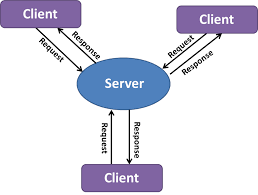
\includegraphics[width=0.3\columnwidth]{client-server.png} 
\caption{Architettura client-server}
\end{figure}
\newpage 
\noindent Nel nostro abbiamo un solo server(anche chiamato Backend) e n client(anche chiamato FrontEnd)
%IMMAGINE 
\begin{figure}[h] 
\centering
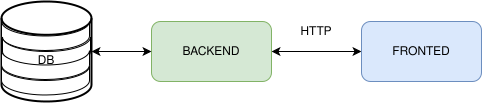
\includegraphics[width=0.6\columnwidth]{client-server2.png} 
\caption{Struttura del progetto}
\end{figure}
\subsection{Backend}
Il Backend è la parte server dell'applicazione responsabile della gestione dei dati.\\
E' stato realizzato in Java mediante l'utilizzo del Framework Spring e un Database H2, in particolare sono state usate le componenti Spring Boot, Spring Web e Spring Data Jpa.
Il primo è un componente di Spring che serve a ridurre il codice di configurazione e permette al programmatore di concentrarsi sulla logica del programma astraendo ulteriormente la complessità di Spring.
\\Il secondo è un componente che serve a creare applicazioni Web.
Nel nostro caso è stato utilizzato per creare un' API Rest che fornisce servizi di gestione dati.
Infine l'ultimo componente serve per la creazione di database relazionali con generazione automatica delle query.
Il backend nel nostro caso è una \textbf{Transaction processing application} ovvero un'applicazione incentrata sui dati che processa le richieste degli utenti(frontend) e aggiorna le informazioni di un database.
%IMMAGINE 
\begin{figure}[h] 
\centering
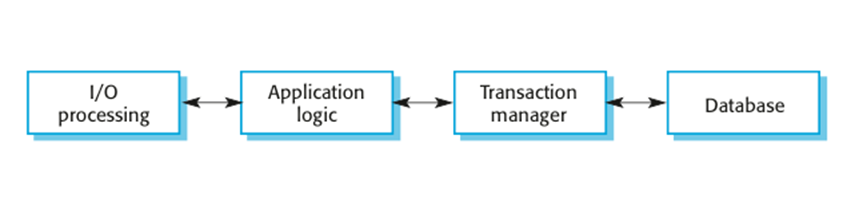
\includegraphics[width=0.8\columnwidth]{logic.png} 
\caption{}
\end{figure}
\\Nello specifico abbiamo utilizzato un' \textbf{Architettura a Strati}:
L'architettura a strati organizza il sistema in strati con ognuno una specifica funzionalità associata ad esso. Uno strato fornisce servizi al livello superiore e utilizza i servizi del livello inferiore.\\
\\Nella nostra applicazione possiamo trovare 4 layer:
%IMMAGINE 
\begin{figure}[h] 
\centering
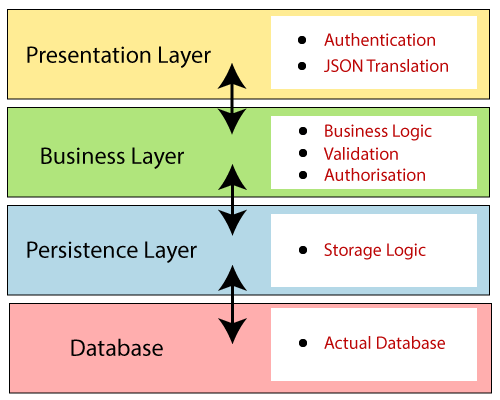
\includegraphics[width=0.4\columnwidth]{spring-boot-architecture.png} 
\caption{}
\end{figure}\\
\textbf{Presentation Layer:} implementato dalle classi Controller ha il compito di gestire le richieste HTTP, tradurre i parametri e il JSON in oggetti.
Infine tutte le informazioni vengono passate al Buisness Layer.\\\\
\textbf{Business Layer:} gestisce la logica di business del programma e la validazione delle richieste, è implementato dalle classi Service e usa i servizi forniti dal Data Access Layer(Persistence Layer).\\\\
\textbf{Persistence Layer:} gestisce la logica dei dati, in altre parole effettua le query e trasforma gli oggetti di buisness(entità) da e in righe del database.\\\\
Oltre alla struttura presentata sopra Spring si basa sul principio di \textbf{Inversion of Control:}
un principio dell'ingegnieria del software che trasferisce il controllo degli oggetti o porzioni di un programma a un container o un framework.\\
In contrasto con la programmazione tradizionale, dove il nostro codice richiama le funzionalità di una libreria, IoC permette al framework di prendere il controllo del flusso di esecuzione ed effetturare chiamate al nostro codice.
\\I principali vantaggi sono:
\begin{itemize}
  \item scorporare l'esecuzione di una funzionalità dalla sua implementazione
  \item rendere facile cambiare implementazione
  \item maggiore modularità nel programma
  \item maggiore facilità nel testing di un programma isolando un componente o mockando le sue dipendenze, permettendo così ai componenti di comunicare mediante contratti
\end{itemize}
Si può implementare questo principio mediante vari meccanismi come:
\begin{itemize}
  \item Strategy design pattern
  \item Service Locator pattern
  \item Factory pattern
  \item Dependency Injection (DI)
\end{itemize}
Ed è proprio quest'ultimo quello usato dal framework.
\subsubsection{Dependency Injection (DI)}
E' un design pattern che possiamo usare per implementare IoC, dove il controllo invertito è quello del settaggio delle dipendenze di un'oggetto.\\
Connettere gli oggetti con altri oggetti, o "inniettare" oggetti dentro altri oggetti, viene fattto da un'assembler invece che dagli oggettti stessi.

%ToDO SPEGA I VARI TIPO https://www.baeldung.com/inversion-control-and-dependency-injection-in-spring

\subsubsection{Spring Bean}
Quando parliamo di DI in Spring non possiamo esimerci dal parlare anche dei Bean. Questi sono gli oggetti che formano la struttura dell'applcazione e che sono gestiti da Spring IoC container.
Un bean è un'oggetto che è istanziato, assemblato e gestito da Spring IoC container. Nel nostro programma i Bean sono i Controller, i Service e le Repository.\\
Ogni Bean inoltre implementa il pattern Singleton.\\

\subsubsection{Singleton}
Il pattern singleton è un meccanismo che assicura che esista solo un'istanza di un oggetto per applicazione.
Generalmente, un singleton è unico globalmente per l'intera applicazione, ma in Spring questo vincolo è "rilassato".\\
Infatti Spring limita un singleton a un oggetto per Spring IoC container.
In pratica, questo significa che Spring creerà solo un Bean di ogni tipo per ogni contesto dell'applicazione.\\
L'approccio di Spring è diverso dalla definizione rigorosa di singleton poiché un'applicazione può avere più di un container Spring. 
Quindi, più oggetti della stessa classe possono esistere in una singola applicazione se abbiamo più contenitori.

\subsection{Frontend}
Il frontend, anche detto Client è la parte grafica del software responsabile dell'interazione con l'utente.
E' stato realizzato in Java mediante l'utilizzo delle librerie JavaFx per la parte Grafica e di Jackson DataBind per il parsing dei dati JSON.\\
Nel nostro caso l'applicazione è un \textbf{Event processing system} ovvero un sistema che risponde agli eventi nell'ambiente del sistema o nell'interfaccia utente.\\
La caratteristica principle dei event processing systems è che la tempistica degli eventi è imprevedibile e il sistema deve essere in grado di far fronte a questi eventi quando si verificano.
Il sistema rileva e interpreta gli eventi. Gli eventi dell'interfaccia utente rappresentano comandi impliciti per il sistema, che esegue alcune azioni per obbedire a quel comando.\\\\
Nello specifico essendo un' applicazione grafica abbiamo usato uno stile architetturale \textbf{Event-driven} ovvero un paradigma di architettura software che promuove la produzione, il rilevamento, il consumo e la reazione agli eventi.\\
Oltre a ciò abbiamo scelto il pattern architetturale \textbf{MVC}.
\subsubsection{Model View Control}
E' un pattern architetturale che separa la rappresentazione e l'interazione dai dati del sistema.
Il sistema è strutturato in tre componenti logiche che interagiscono tra loro.
\begin{itemize}
  \item \textbf{Model:} gestisce i dati di sistema e le operazioni associate su
quei dati
  \item \textbf{View:} definisce e gestisce il modo in cui i dati sono presentati all'utente
    \item \textbf{Control:} gestisce l'interazione dell'utente (ad esempio, pressioni di tasti, clic del mouse, ecc.) e passa queste interazioni alle altre componenti
\end{itemize}
\newpage
%IMMAGINE 
\begin{figure}[h] 
\centering
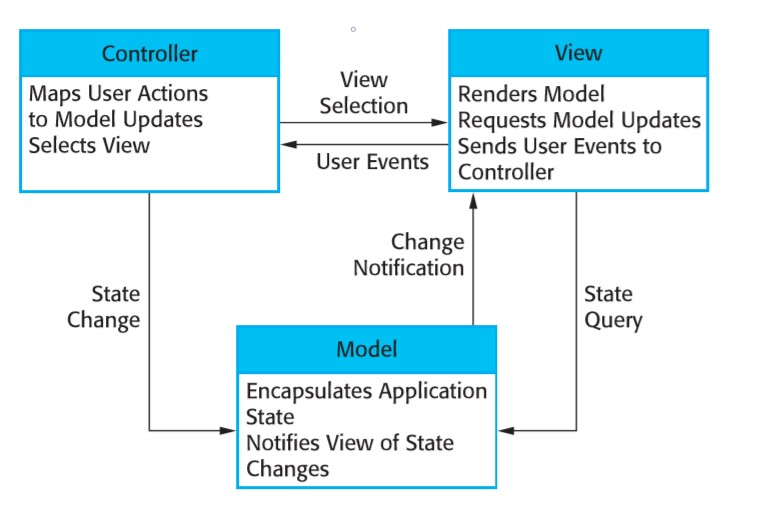
\includegraphics[width=0.5\columnwidth]{MVCdiagram.png} 
\caption{}
\end{figure}
\\Nel nostro progetto il controller corrisponde alle classi Controller, la View ai file FXML e il model alle entitites.\\
Come ultima cosa il frontend utilizza Dependecy Injection per inniettare i componenti grafici nel controller e degli oggetti Singleton chiamati TempMemory e UserTempMemory per trasferire i dati tra un controller e l'atro.
\section{Progetto dell’architettura ed implementazione del database}
Per lo sviluppo del sistema è stato un database relazione H2 su file e la libreria Spring Data JPA per interfacciare il sistema al Database. La logica del database é stata di tipo icrementale seguita da numerosi refactor per implementare nuove funzionalitá ,questo ha portato al non seguire uno schema logico.Di sotto possiamo trovare un piccolo schema del attuale database. 
%IMMAGINE 
\begin{figure}[h] 
\centering
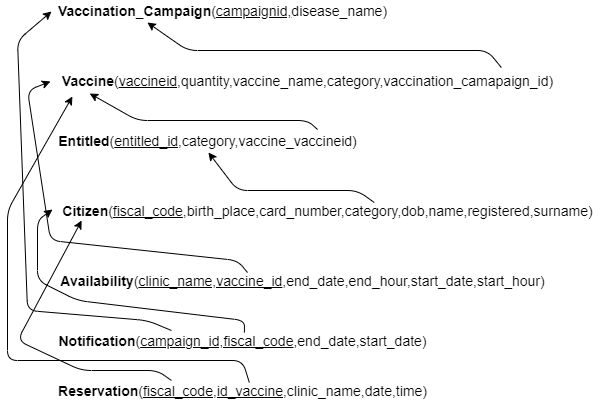
\includegraphics[width=0.5\columnwidth]{logicDB.png} 
\caption{Schema Logico del Database}
\end{figure}
\newpage
\chapter{Attivita di test e validatione}
\section{Generalitá}
Il test ha lo scopo di dimostrare che un software fa quello che è destinato a fare e scoprirne i difetti prima che venga messo in uso. 
Esistono 3 fasi del processo di test:
\begin{itemize}
  \item \textbf{Development testing: }dove il sistema viene testato durante lo sviluppo per scoprire bug e difetti.
  \item \textbf{Release testing: }dove un team di test separato prova la versione completa del sistema prima che venga rilasciato agli utenti.
    \item \textbf{User testing: }dove utenti o potenziali utenti di un sistema testano il sistema nel proprio ambiente.
\end{itemize}
\section{Development Testing}
I test di sviluppo includono tutte le attività di test che sono svolte dal team che sviluppa il sistema. Nel nostro caso i test automatici sono stati eseguiti solo per il backend in quanto non avevamo abbastanza tempo per effettuarli anche sul fronted.\\
Questi sono a loro volta divisi in 3 parti:
\begin{itemize}
  \item \textbf{Unit testing: }dove si testano singole unità del programma o classi.\\Questi test si concentrano sul verificare le funzionalità di singoli oggetti o metodi.
  \item \textbf{Component testing: }anche detti Integration testing, qua sono integrate diverse unità individuali per creare componenti compositi
    \item \textbf{System testing: }anche chiamati Acceptance testing qui tutti i componenti di un sistema sono integrati e il sistema viene testato nel suo insieme.
\end{itemize}
Per effettuare questi test abbiamo utilizzato 3 librerie:
\begin{itemize}
  \item \textbf{Junit5: }è al centro dell'infrastruttura di testing e serve principalmente come base per definire le funzioni di test, funzioni di supporto e le classi di test mediante le apposite annotazioni.
  \item \textbf{Mockito: }consente la creazione di oggetti fittizi(mock object), al fine di predefinire il comportamento di un'oggetto in modo da poter testare gli oggetti singolarmente senza le loro dipendenze.
    I \textbf{mock object} sono oggetti simulati che imitano il comportamento di oggetti reali in maniera controllata. Un programmatore in genere crea un oggetto fittizio per testare il comportamento di qualche altro oggetto, più o meno allo stesso modo in cui un progettista di automobili utilizza un manichino per crash test per simulare il comportamento dinamico di un essere umano negli impatti di un veicolo.
    \item \textbf{AssertJ: } è una libreria per semplificare la scrittura e migliorare la leggibilità delle asserzioni nei test. 
    Un'\textbf{asserzione} è un'espressione che incapsula una logica verificabile specificata su un obiettivo sottoposto a test.
\end{itemize}
Inoltre anche durante i test è stato utilizzato il pattern Dependecy Injection per inniettare le dipendenze e gli oggetti fittizi nelle classi di test.
\section{Unit testing}
In questi test abbiamo testato le classi senza avviare il framework e scorporando le dipendenze mediante mockito. Per effettuare questi test abbiamo seguito il paradigma \textbf{given-when-then}, tale paradigma consiste nella suddivisione del codice di test in tre blocchi:
\begin{itemize}
  \item \textbf{given:} in questo blocco mettiamo il sistema in uno stato noto definendo i dati di partenza e il comportamento delle componenti fittizzie.
  \item \textbf{when:} in questo blocco vengono descritte le operazioni compiute dall'utente
    \item \textbf{then:} questo è il blocco di verifica, osserviamo l'output del sistema e controlliamo se si è comportato come ci aspettiamo.
\end{itemize}
Oltre a questo abbiamo seguito una convenzione per i nomi delle funzioni in modo da rendere i metodi "parlanti" ovvero autoesplicativi.\\
Infatti tutti i metodi di test seguono questa struttura del nome:\\
\textit{\color{red}nomeDelMetodoCheStoTestando\_StatoDuranteIlTest\_CosaMiAspetto\((\))}\\
\\Adesso analizziamo alcuni dei test scritti, iniziando dalla classe da testare.
\\Per lo scopo di questa documentazione il codice di seguito esposto è solo un'estrapolazione del codice reale.
\begin{lstlisting}[language=Java]
@Service
@AllArgsConstructor
public class VaccineService {
	private final VaccineRepository vaccineRepository;

	public Vaccine addQuantity(Long vaccineID, Long quantity) {
	 Optional<Vaccine> optionalVaccine = vaccineRepository.findById(vaccineID);
		Vaccine vaccine;
		if (optionalVaccine.isPresent())
			vaccine = optionalVaccine.get();
		else
			throw new IllegalStateException("Insert a Valid ID");

		if (quantity < 0)
			throw new IllegalStateException("Insert a Valid quantity");

		vaccine.setQuantity(vaccine.getQuantity() + quantity);
		return vaccineRepository.save(vaccine);
	}
}
\end{lstlisting}
L'annotazione \textit{@Service} serve ad indicare a Spring che questo è un bean di tipo Service, la successiva annotazione \textit{@AllArgsConstructor} è un'annotazione della libreria \textit{LomBok} che serve ad indicare alla libreria di creare automaticamente un costruttore con tutti gli argomenti.
\\Quel costruttore verrà utilizzato per inniettare l'oggetto \textit{VaccineRepository} dentro la variabile.\\
Come vediamo la funzione \textit{addQuantity} accetta 2 parametri: l'Id del Vaccino e di quanto aumentare la quantità e ritorna un'oggetto \textit{Vaccine} con l'id corrispondente a quello passato ma la quantità di quel vaccino verrà aumentata di quanto richiesto.\\
Tale funzione fallisce in soli 2 casi se l'id del vaccino richiesto non è presente nel Database oppure se la quantità inserita è inferiore a 0.\\
\\Ora passiamo ad analizzare i metodi di test:
\begin{lstlisting}[language=Java]
@ExtendWith(MockitoExtension.class)
class VaccineServiceUnitTest {
    @Mock
    private VaccineRepository vaccineRepository;
    private VaccineService underTest;
    private Vaccine vaccine;

    @BeforeEach
    void setUp() {
        this.underTest = new VaccineService(vaccineRepository);
        this.vaccine = new Vaccine(
                8L,
                "jansen",
                100L
        );
    }
}
\end{lstlisting}
Quella presentata sopra è un pezzo di codice comune a tutti i metodi che presenteremo tra poco essendo i metodi parte della classe VaccineServiceUnitTest.\\
La classe è annotata con \textit{@ExtendWith(MockitoExtension.class)} tale annotazione indica al motore di test di avviare mockito così da poter successivamente inniettare un'oggetto mockato mediante l'annotazione \textit{@Mock}.\\
Troviamo inoltre una funzione setUp annotata \textit{@BeforeEach} che indica al motore di test di avviare quel metodo di supporto prima di ogni metodo di test.\\
\begin{lstlisting}[language=Java]
@Test
void addQuantity_validQuantity_pass() {
    // given
    Long id = vaccine.getVaccineID();
    given(vaccineRepository.findById(id)).willReturn(Optional.of(vaccine));
    given(vaccineRepository.save(any(Vaccine.class))).willAnswer(invocationOnMock -> invocationOnMock.getArgument(0));

    // when
    Vaccine result = underTest.addQuantity(id, 50L);

    // then
    BDDMockito.then(vaccineRepository).should(times(1)).save(any());
    BDDAssertions.then(result.getQuantity()).isEqualTo(150L);
}
\end{lstlisting}
Quella sopra presentata è la prima funzione di test, possiamo notare tale fatto dall'annotazione \texttit{@Test}.
Tale funzione andrà a testare il metodo \texttit{addQuantity} passandogli una quantità valida e tale test dovrebbe passare.
Ciò è facilmente deducibile grazie alla naming convention scelta la quale ci descrive cosa fa la funzione.\\
Passando al codice nel blocco \textbf{given} come detto prima definiamo un'ambiente controllato, specificatamente in questo caso definiamo il comportamento di \texttit{vaccineRepository.findById} la quale dovrebbe ritornale un'oggetto optional contenente il vaccino inizializzato dal metodo \texttit{setUp} e del metodo \textit{vaccineRepository.save} il quale dovrà restituire l'oggetto passato.\\
Successivamente nel blocco \textbf{when} definiamo il comportamento dell'utente ovvero quello di chiamare il metodo \textit{addQuantity}.\\
Infine nel blocco \textbf{then} andiamo a verificare l'output, controllando che la funzione save venga chiamata 1 volta e che l'oggetto che ci viene restituito abbia una quantità di 150.\\
\noindent
\begin{lstlisting}[language=Java]
void addQuantity_quantitySmallerThanZero_throwException() {
    // given
    long quantity = -5;

    given(vaccineRepository.findById(vaccine.getVaccineID())).willReturn(
            Optional.of(vaccine)
    );

    // when
    final Throwable throwable = catchThrowable(() -> underTest.addQuantity(vaccine.getVaccineID(), quantity));

    // then
    BDDAssertions.then(throwable)
            .isInstanceOf(IllegalStateException.class)
            .hasMessage("Insert a Valid quantity");

    BDDMockito.then(vaccineRepository).should(never()).save(any());
}
\end{lstlisting}
Questa seconda funzione andrà sempre a testare la funzione addQuantity ma verificandone il comportamento quando la quantità passata è inferiore a 0.\\
Passando al codice nel blocco \textbf{given} esso è uguale a quello precedente ma la differenza è che la quantità è definita come un valore negativo.\\
Successivamente nel blocco \textbf{when} definiamo il comportamento dell'utente ovvero quello di chiamare il metodo \textit{addQuantity} e salviamo l'eccezione che verrà lanciata all'interno di una variabile .\\
Infine nel blocco \textbf{then} andiamo a verifiare l'output, controllando che la funzione save non venga mai chiamata e che l'eccezione che viene lanciata sia come ci aspettiamo.\\
\begin{lstlisting}[language=Java]
void addQuantity_IdDoesNotExist_throwError() {
    // given
    given(vaccineRepository.findById(anyLong())).willReturn(Optional.empty());

    // when
    final Throwable throwable = catchThrowable(() -> underTest.addQuantity(vaccine.getVaccineID(), 50L));
    // then
    BDDAssertions.then(throwable)
            .isInstanceOf(IllegalStateException.class)
            .hasMessage("Insert a Valid ID");

    BDDMockito.then(vaccineRepository).should(never()).save(any());
}
\end{lstlisting}
Questa ultima funzione andrà sempre a testare la funzione addQuantity ma verificandone il comportamento quando l'id passato non è presente nel database.\\
Passando al codice nel blocco \textbf{given} come detto prima definiamo un'ambiente controllato, specificatamente in questo caso definiamo il comportamento di \textit{vaccineRepository.findById} la quale dovrebbe ritornare un'oggetto optional vuoto segno del fatto che non vi è presente alcun Vaccino con l'id richiesto nel Database.\\
Successivamente nel blocco \textbf{when} definiamo il comportamento dell'utente ovvero quello di chiamare il metodo \textit{addQuantity} e salviamo l'eccezione che verrà lanciata all'interno di una variabile \\
Infine nel blocco \textbf{then} andiamo a verifiare l'output, controllando che la funzione save non venga mai chiamata e che l'eccezione che viene lanciata sia come ci aspettiamo.\\
Con questi tre semplici metodi abbiamo testato completamente la funzione in ogni suo posssibile caso.
\section{Integration testing}
Questi test sono stati eseguiti solo sui Controller, a differenza degli Unit Test qui abbiamo avviato il framework ma comunque abbiamo scorporato le dipendenze così da poter testare il corretto parsing dei dati Json.\\\\
Vediamo di seguito la classe che andremo a testare:
\begin{lstlisting}[language=Java]
@RestController
@AllArgsConstructor
@RequestMapping(path = "/citizens")
public class CitizenController {
    private final CitizenService citizenService;

    @GetMapping
    public CitizenWrapper getCitizens() {
        return new CitizenWrapper(
                citizenService.getCitizens()
        );
    }
}
\end{lstlisting}
L'annotazione \textit{@RestControlle}r serve ad indicare a Spring che questo è un bean di tipo Controller, la successiva annotazione \textit{@AllArgsConstructor} è un'annotazione della libreria \textit{LomBok} che serve ad indicare alla libreria di creare automaticamente un costruttore con tutti gli argomenti.\\Quel costruttore verrà utilizzato per inniettare l'oggetto CitizenService dentro la variabile.\\L'ultima annotazione \textit{@RequestMapping} indica su quale endpoint andranno mappati i successivi metodi. Il metodo che andremo a testare è \textit{getCitizens} il quale serve per ottenere una lista di tutti i cittadini presenti nel sistema. Tale metodo è annotato con \textit{@GetMapping} tale annotazione serve ad indicare a spring che questo metodo sarà responsabile della gestione delle richieste GET sull'endpoint precedententemente specificato. La funzione semplicemente restituisce un'oggetto \textit{CitizenWrapper} contenente la lista dei cittadini la quale ci viene restituita da \textit{citizenService.getCitizens().}\\
\newpage
\noindent Ora passiamo ad analizzare i test veri e propri partendo dalla struttura generale:
\begin{lstlisting}[language=Java]
@ExtendWith(SpringExtension.class)
@WebMvcTest(controllers = CitizenController.class)
class CitizenControllerIntTest {
    private final static String URI = "/citizens";

    private Citizen citizen;
    private String fiscalCode;

    @Autowired private MockMvc mockMvc;
    @Autowired private ObjectMapper objectMapper;
    @MockBean private CitizenService citizenService;


    @BeforeEach
    void setUp() {
        fiscalCode = "MZZMMT61M22D854K";
        citizen = new Citizen(
                fiscalCode,
                237971319838010581L,
                "Mouhameth",
                "Mazza",
                "Gaiarine",
                LocalDate.parse("1961-08-22"),
                "paziente iperteso"
        );
    }
}
\end{lstlisting}
La prima annotazione serve ad avviare Junit mentre la seconda ad avviare parte del contesto di Spring e a specificare a quale classe si riferisce questo test.\\
Continuando possiamo notare dei campi annotati con \textit{@Autowired e @MockBean}, la prima serve a dire a Spring di inniettare i Bean, la seonda invece serve per dire a Mockito di creare un'oggetto fittizio e aggiungerlo al contesto di Spring così che possa essere iniettato nel campo.
\\Infine all'inteno della funzione setUp andiamo a definire alcuni dati che dopo verranno usati per effettuare i test.\\\\
Vediamo ora un metodo di test:
\begin{lstlisting}[language=Java]
@Test
void getCitizens_shouldCallService() throws Exception {
    mockMvc.perform(get(URI)).andExpect(status().isOk());
    verify(citizenService).getCitizens();
}
\end{lstlisting}
Nella prima riga effettuiamo una richiesta GET all'endpoint specificato nella variabile URI e definiamo i parametri secondo coi la richiesta è andata a buon fine, nello specifico ci aspettiamo che la richiesta HTTP finisca con uno status code 200(OK).\\
Sotto verifichiamo che la funzione getCitizens sia stata chiamata a seguito della richiesta HTTP.
\newpage
\section{Acceptance testing}
Questi test sono stati eseguiti solo sui Controller, all'apparenza possono sembrare uguali agli Integration Test ma la differenza sostanziale è che qui viene avviato l'intero applicativo senza scorporare le dipendenze e quindi andiamo a testare il sistema nel suo insieme.\\
Vediamo di seguito la classe che andremo a testare:
\begin{lstlisting}[language=Java]
@RestController
@AllArgsConstructor
@RequestMapping(path = "/citizens")
public class CitizenController {
    private final CitizenService citizenService;

    @GetMapping(path = "/{fiscalCode}")
    public Citizen getCitizen(@PathVariable String fiscalCode) {
        return citizenService.getCitizen(fiscalCode);
    }
}
\end{lstlisting}
Le annotazioni della classe sono le stesse viste in precenza, queste servono a definire il tipo di Bean , a creare il costruttore e definire l'endpoint. In questo caso rispetto al codice mostrato in precedenza notiamo che l'annotazione @GetMapping  è più complessa infatti viene definito un'attributo dell'annotazione chiamato path il cui valore è "/{fiscalCode}" questo valore indica che il valore inserito dopo lo "/" andrà inserito nella variabile fiscalCode, inoltre questo path andrà a sommarsi dopo il path definito sopra la classe.
Per capire meglio facciamo un'esempio, supponiamo che il nostro url sia il seguente:
\underline{http://localhost:8080/citizens/BRTCRL30A29E684P}
Come possiamo notare dopo /citizens/ abbiamo inserito un valore, questo sarà il valore che andrà inserito nella variabile fiscalCode.
Per capire meglio facciamo un'esempio, supponiamo che il nostro url sia il seguente:
\underline{http://localhost:8080/citizens/BRTCRL30A29E684P}
Come possiamo notare dopo /citizens/ abbiamo inserito un valore, questo sarà il valore che andrà inserito nella variabile fiscalCode.
Andando ad analizzare il corpo della funzione semplicemente questa richiama e ritorna il valore della funzione \textit{getCitizen} di CitizenService passandole come parametro il contenuto della variabile fiscalCode. Andando ad analizzare il corpo della funzione semplicemente questa richiama e ritorna il valore della funzione \textit{getCitizen} di CitizenService passandole come parametro il contenuto della variabile fiscalCode.\\
\newpage
\noindent Ora passiamo ad analizzare i test veri e propri partendo dalla struttura generale:
\begin{lstlisting}[language=Java]
@ExtendWith(SpringExtension.class)
@SpringBootTest
@AutoConfigureMockMvc
class CitizenControllerAcceptanceTest {
    private final static String URI = "/citizens";

    private Citizen citizen;
    private Citizen citizen2;
    private String fiscalCode;

    @Autowired private MockMvc mockMvc;
    @Autowired private ObjectMapper objectMapper;
    @Autowired private CitizenRepository citizenRepository;

    @BeforeEach
    void setUp() {
        fiscalCode = "MZZMMT61M22D854K";
        citizen = new Citizen(
                fiscalCode,
                237971319838010581L,
                "Mouhameth",
                "Mazza",
                "Gaiarine",
                LocalDate.parse("1961-08-22"),
                "paziente iperteso"
        );
        citizen2 = new Citizen(
                "NNCFNC59C67E709B",
                963231202896772494L,
                "Francesca Amira",
                "Innocenti",
                "Lozzo Atestino",
                LocalDate.parse("1959-03-27"),
                "paziente oncologico"
        );
    }

    @AfterEach
    void tearDown() {
        citizenRepository.deleteAll();
    }
}
\end{lstlisting}
Nel codice sovraesposto andiamo ad avviare Spring e Junit oltre a definire alcuni oggetti che usermo per i test.
Inoltre abbiamo definto un metodo \textit{tearDown} il cui compito è quello di ripulire la tabella del db.
Tale metodo è annotato con \textit{@AfterEach} questa annotazione inca a Junit che il metodo deve essere eseguito dopo ogni metodo di test.\\
\newpage \noindent Vediamo ora un metodo di test:
\begin{lstlisting}[language=Java]
@Test
void getCitizen_shouldReturnCitizen() throws Exception {
    citizenRepository.saveAll(List.of(citizen,citizen2));

    MvcResult result = mockMvc.perform(get(URI+"/"+fiscalCode)).andExpect(status().isOk()).andReturn();
    String response = result.getResponse().getContentAsString();
    assertThat(response).isEqualToIgnoringWhitespace(objectMapper.writeValueAsString(citizen));
}
\end{lstlisting}
Nella prima riga mettiamo il sistema in uno stato noto salvando nel database due cittadini, in seguito effettuiamo una richiesta GET e definiamo i parametri secondo coi la richiesta è andata a buon fine, nello specifico ci aspettiamo che la richiesta HTTP finisca con uno status code 200(OK). 
Inoltre vogliamo che il valore della risposta ci sia ritornato e che venga salvato in una variabile.
Infine controlliamo che la stringa di risposta corrisponda a ciò che ci aspettiamo.
\subsection{Release testing}
Per la fase di Release testing abbiamo fatto testare il software ad altri sviuppatori nostri colleghi i quali oltre a verificare la corretta funzionalità del software ci hanno fato alcuni consigli per migliorare la qualità del codice.\\
\subsection{User testing}
Come ultimo scaglione il software è stato sottoposto ad un breve test da parte di alcuni individui con limitata dimestichezza informatica. In questa fase non si è cercato in nessun modo di guidare o strutturare l’esperienza, per non influenzare in alcun modo il risultato; piuttosto si è lasciato che il soggetto navigasse liberamente il sistema. E' stata fornita l'oro solo una breve descrizione dello scopo del software. L'unico scopo del test era quello di individare errori e migliorare la User Experience.\\
Grazie a quest'ultimo test sono state inoltre individuate anche alcune funzionalità aggiuntive per il software tra cui:
\begin{itemize}
\item la possibilità per il personale ASL di registrare al sistema nuovi Utenti
\item la possibilità per il personale ASL di aggiungere dall'interfaccia altre categorie oltre a quelle preesistenti
\item la possibilità per il personale ASL di aggiungere delle sedi dall'interfaccia e successivamente durante l'aggiunta delle disponibilità scegliere la sede tra un'insieme finito di possibilità inceve che doverne digitare il nome
\end{itemize}
\newpage
\chapter{Biblografia}
\begin{itemize}
\item\url{https://www.javatpoint.com/spring-boot-architecture}
\item\url{https://www.baeldung.com/spring-vs-spring-boot}
\item\url{https://www.baeldung.com/spring-bean}
\item\url{https://www.baeldung.com/spring-framework-design-patterns}
\item\url{https://www.baeldung.com/inversion-control-and-dependency-injection\\-in-spring}
\item\url{https://ifs.host.cs.st-andrews.ac.uk/Books/SE9/Web/Architecture/AppArch/EventProc.html}
\item\url{https://en.wikipedia.org/wiki/Event-driven_architecture}
\item\url{https://en.wikipedia.org/wiki/Mock_object}
\item\url{https://en.wikipedia.org/wiki/Mockito}
\item\url{https://www.vogella.com/tutorials/AssertJ/article.html}
\item\url{https://blog.j-labs.pl/index.php?page=2017/02/Given-When-Then-pattern\\-in-unit-tests}
\item Ian Sommerville. 2015. Software Engineering (10th. ed.). Pearson.
\end{itemize}
\end{document}
